% BAC 2022 D - Exercice 4
% Courbe de f(x) = -(x+1)e^{-x} - 1

\documentclass[border=5pt]{standalone}
\usepackage{pgfplots}
\usepackage{amsmath}
\usepackage{amssymb}

\begin{document}

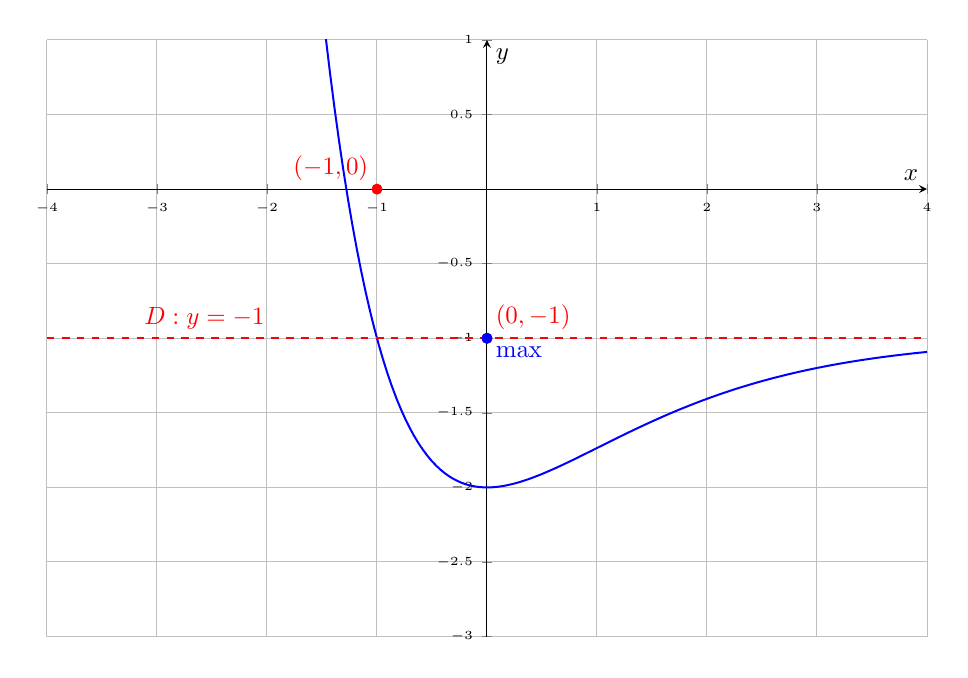
\begin{tikzpicture}[scale=0.9]
\begin{axis}[
    width=14cm,
    height=10cm,
    axis lines=center,
    xlabel=$x$,
    ylabel=$y$,
    xmin=-4, xmax=4,
    ymin=-3, ymax=1,
    grid=major,
    samples=200,
    legend pos=outer north east,
    tick label style={font=\tiny}
]

% Function f(x) = -(x+1)*exp(-x) - 1
\addplot[blue, thick, domain=-4:4] {-(x+1)*exp(-x) - 1} 
    node[pos=0.3, below right] {$\Gamma$};

% Horizontal asymptote at y = -1 (lim x -> +inf)
\addplot[red, dashed, thick, domain=-4:4] {-1} 
    node[pos=0.1, above right] {$D: y=-1$};

% Tangent at origin
% f'(x) = xe^(-x), f'(0) = 0
% Tangent is horizontal at origin

% Point h(0) = -1
\addplot[mark=*, red] coordinates {(0,-1)} 
    node[above right] {$(0,-1)$};

% Point h(-1) = 0
\addplot[mark=*, red] coordinates {(-1,0)} 
    node[above left] {$(-1,0)$};

% Maximum (f'(x) = 0 when x = 0)
\addplot[mark=*, blue] coordinates {(0,-1)} 
    node[below right] {max};

\end{axis}

\end{tikzpicture}

\end{document}